\chapter{Performance and Analysis}
\renewcommand{\baselinestretch}{\mystretch}
\label{chap:Perf}
%\setlength{\parindent}{0pt}

\section{Platform comparison}

\fref{fig:raw-seq-p-c} clearly shows the relative performance figures of all testing platforms. The NP1380 platform is unable to meet the minimum requirement of 50 fps sequences, therefore most performance analysis for \texttt{VixenConsole} was done on the Raspberry Pi B+ platform.

\section{Implementation comparison}

\begin{figure}[!t]
  \centering
  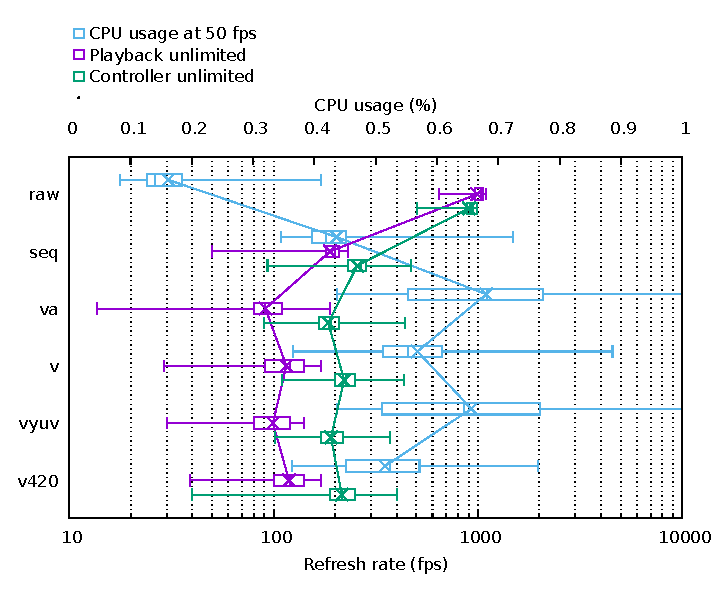
\includegraphics[width=0.8\textwidth]{Figs/RPi-perf.eps}
  \caption{\footnotesize Performances of different implementations on Raspberry Pi B+}
  \label{fig:perf-RPi}
\end{figure}

\fref{fig:perf-RPi} shows the performance comparison between different implementations on Raspberry Pi B+. \texttt{VixenLinky} (referenced by \texttt{raw}) has the highest refresh rate for its simplicity. \texttt{VixenConsole} with the ``Raw'' sequence format (referenced by \texttt{seq}) has the second highest performance. The unlimited playback performance drops to almost half when using a \texttt{rgb24} encoded video as the input (referenced by \texttt{v}). The performance drops again by a small factor when audio stream was also added to the video input (referenced by \texttt{va}). The video only playback performance of \texttt{yuv420p} encoding (referenced by \texttt{v420}) is only a little bit higher than the lossless \texttt{rgb24} encoding (\texttt{v}), whereas the performance of lossless \texttt{yuv444p} encoding (referenced by \texttt{vyuv}) is noticeably lower. Therefore, video encoding format of \texttt{libx264rgb} with \texttt{rgb24} pixel format is more suitable for encoding video sequences.

\cmt{Test different container formats?}

\begin{figure}[!t]
  \centering
  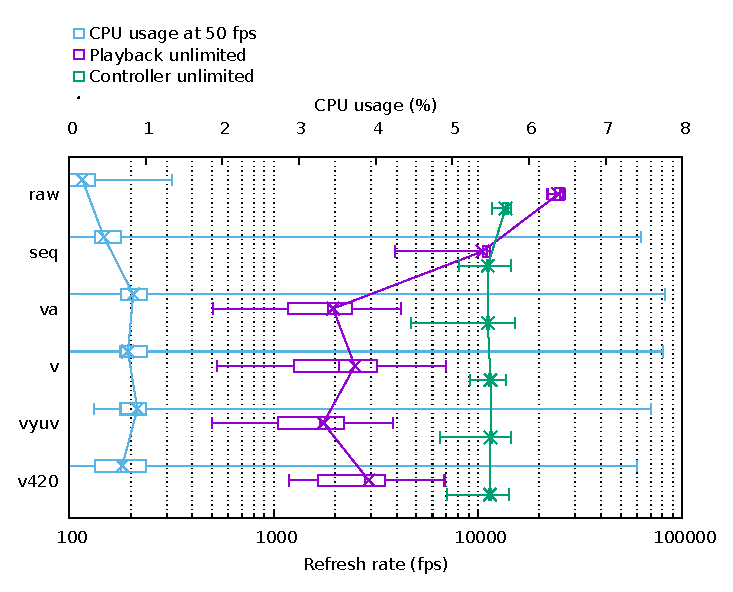
\includegraphics[width=0.8\textwidth]{Figs/TX2-perf.eps}
  \caption{\footnotesize Performances of different implementations on Jetson TX2}
  \label{fig:perf-TX2}
\end{figure}

\fref{fig:perf-TX2} shows the performance comparison on the NVIDIA Jetson TX2 platform. This platform has similar single core CPU performance to the Microsoft Windows laptop. The maximum refresh rates easily reaches over 1,000 fps for playback and 10,000 fps for controllers. For the 50 fps sequence, the CPU usage almost never reaches above $1 \%$. Compare to the original Vixen application struggling to maintain a stable 50 fps refresh rate on Microsoft Windows, the new playback engine definitely achieved incomparable performance improvements.
